\documentclass[10pt,twocolumn,letterpaper]{article}

\usepackage{cvpr}
\usepackage{float}
\usepackage{times}
\usepackage{epsfig}
\usepackage{graphicx}
\usepackage{amsmath}
\usepackage{amssymb}
\usepackage{caption}
\usepackage{subcaption}
\usepackage{tikz}
\usepackage{pgfplots}
\pgfplotsset{compat=newest}
\usepgfplotslibrary{units}
\pgfplotsset{width=10cm,compat=1.9}
\usepgfplotslibrary{external}
\tikzexternalize
\usepackage[backend=bibtex,
style=numeric,
bibencoding=ascii
%style=alphabetic
%style=reading
]{biblatex}
\addbibresource{bibliography.bib}

% Include other packages here, before hyperref.

% If you comment hyperref and then uncomment it, you should delete
% egpaper.aux before re-running latex.  (Or just hit 'q' on the first latex
% run, let it finish, and you should be clear).
\usepackage[breaklinks=true,bookmarks=false]{hyperref}

\cvprfinalcopy % *** Uncomment this line for the final submission

\def\cvprPaperID{****} % *** Enter the CVPR Paper ID here
\def\httilde{\mbox{\tt\raisebox{-.5ex}{\symbol{126}}}}

\begin{document}

%%%%%%%%% TITLE
\title{ATML Project Report: X-rays Bone age Prediction}

\author{Lukas Zbinden\\
University of Fribourg\\
ATML course, University of Bern, Spring 2018\\
{\tt\small lukas.zbinden@unifr.ch}
}

\maketitle
%\thispagestyle{empty}

%-------------------------------------------------------------------------
%%%%%%%%% ABSTRACT
\begin{abstract}
   Our project took on the challenge of skeletal age prediction based on pediatric hand X-rays. We aimed at improving existing baselines by enhancing them with techniques including image preprocessing, transfer learning using a dataset from a different domain and the use of different architectures, respectively, and then analyzing the impact of each approach on the prediction performance. Apart from noneffective results some of our experiments provided hints towards improving the prediction performance.
\end{abstract}

%%%%%%%%% BODY TEXT
\section{Introduction}
In 2017 the Radiological Society of North America (RSNA) published a pediatric bone age prediction challenge (\cite{rsnacompetition}) that asked the ML community to develop an algorithm that most accurately determines skeletal age on a test set of pediatric hand radiographs. The competition was won by \cite{16bitrsnachallenge} with a mean absolute difference (MAD) of 4.265 months. Following that, \cite{kaggleboneage} published the bone age data set on kaggle.com along with a strong baseline algorithm for further exploration and research. That is where we as group 3 stepped in to pick up this baseline and build on it with new ideas and unprecedented experiments.\\ We focused on three areas, namely the impact of different image preprocessing techniques, transfer learning with a different dataset as well as the use of different architectures, respectively, on the prediction task.

%-------------------------------------------------------------------------
\section{Related work}
We mainly focused on the work in \cite{kaggleboneage} and Kevin Mader, respectively, which we used as the baseline for our experiments. Further, we attempted to rebuild the competition winner's model according to \cite{16bitrsnachallenge} which we also used as a reference for our experiments. The techniques we applied in our work, such as data augmentation, in particular histogram equalization, as well as transfer learning are all based on prior contributions by the ML research community (e.g. \cite{1411.1792}). \\
Fundamental to our work were two sets of images, namely the Stanford medicine bone age dataset (\cite{stanfordboneage}) as the main source for the prediction task and the large NIH chest dataset (\cite{nihchestxray}) for experiments with transfer learning. See figure \ref{fig:imgdss} for examples.

\begin{figure}[h]
\centering
\begin{subfigure}{0.2\textwidth}
\includegraphics[width=1.0\linewidth]{images/sample_boneage.png} 
\caption{Stanford bone age}
\label{fig:subim1}
\end{subfigure}
\begin{subfigure}{0.2\textwidth}
\includegraphics[width=1.0\linewidth]{images/sample_chest.png}
\caption{NIH chest}
\label{fig:subim2}
\end{subfigure}
\caption{Dataset samples}
\label{fig:imgdss}
\end{figure}


%------------------------------------------------------------------------
\section{Our methods}
We proposed a set of methods to apply and experiment with over the baseline and study the impact on the prediction performance. Subsequently each of them is briefly introduced.

\subsection{Image preprocessing}
The idea was to preprocess the bone age images in various ways the programming framework would support in order to augment the dataset for better training. Further we wanted to explore the effects of using image histogram equalization with the idea that increased contrast would lead to increased details and therefore a more valuable image for the training process.

\subsection{Rebuilding the 16bit competition winner}
One approach was to rebuild the winner's model 16BitNet of the 2017 RSNA ML challenge as close as possible according to \cite{16bitrsnachallenge} which uses the \verb+InceptionV3+ architecture (cf. figure \ref{fig:16bitnet}). And then use that model as a starting point for our experiments. Note that this model not only has the X-rays image as input but also the respective patient's gender.

\begin{figure}[h]
\includegraphics[scale=0.2]{images/16BitNet.png}
\centering
\caption{16BitNet architecture}
\label{fig:16bitnet}
\end{figure}

\subsection{Use of different architectures}
Additionally, an idea was to apply a set of different networks to the 16BitNet model (\cite{16bitrsnachallenge}) and replace their network choice of \verb+InceptionV3+ while maintaining the same architecture. See figure \ref{fig:SeResNet50} for an example with the SeResNet50 network.

\begin{figure}[h]
\includegraphics[scale=0.6]{images/SeResNet50_arch.png}
\centering
\caption{SeResNet50 architecture}
\label{fig:SeResNet50}
\end{figure}

For the experiments we reused this architecture as the basis but with different networks at the beginning.

\subsection{Transfer learning}
One approach was to train the model on the large NIH chest X-rays data set and then to transfer the weights to the model for bone age prediction on the much smaller Stanford bone age dataset. 
To the best of our knowledge this had not been attempted before which was also confirmed by Kevin Mader. We devised a set of experiments outlined in table \ref{table:taexp}.

\begin{table}[h]
\begin{center}
\begin{tabular}{|c|l|}
\hline
Nr & Experiment \\
\hline\hline
1 & Validate chest X-rays against disease or age \\
2 & Only chest samples within bone age range \\
3 & Use different number of fixed model layers \\
4 & Difference if model pretrained on ImageNet \\
5 & Does adding gender as input improve the result? \\
6 & Regression vs. Classification on age \\
7 & Pretrain baseline \cite{kaggleboneage} with NIH chest dataset \\
\hline
\end{tabular}
\end{center}
\caption{Our transfer learning experiments}
\label{table:taexp}
\end{table}


%-------------------------------------------------------------------------
\section{Experiments}
We evaluated the effects of our proposed methods and subsequently present the findings.

\subsection{Implementation details}
All models were trained using Keras \cite{keras} on 1 GPU on node03 server for 5 epochs (due to time restrictions and contention on the GPU resource between three team members). The learning rate was kept constant until it reached a plateau where it was decreased by a factor of 0.8. We used an initial learning rate of 0.001 to train the models and a default image size of 299x299 unless otherwise stated, the Adam optimizer for default model training and the SGD optimizer for finetuning. As mostly deep models were used, we repeatedly faced problems with \verb+ResourceExhaustedError+ as these consume much memory and tried with \verb+backend.clear_session()+ which also caused crashes of other kinds. Repeated execution usually helped us to eventually progress. 

\subsection{Datasets}
As mentioned earlier, where not stated otherwise, we used the Stanford medicine bone age dataset \cite{stanfordboneage} to run our experiments and additionally for the transfer learning tests we used the NIH chest dataset \cite{nihchestxray} with a total of 112,120 images. The partitioning of the boneage dataset is 12,612 images for the training set, 1,426 images for the validation set and 200 for the test set (three different sets were provided).

\subsection{Image preprocessing}
We tried an array of parameters supported by Keras' \verb+ImageDataGenerator+ but with no noteworthy effects on the results.\\
Then we explored histogram equalization using the function \verb+equalize_adapthist()+ provided by scikit-learn. The effects of this method on an image are depicted in figure \ref{fig:fighistx}. As can be seen in figure \ref{fig:fighistd}, pixels not well represented get more weight and vice versa.

\begin{figure}[h]
\centering
\begin{subfigure}{0.2\textwidth}
\includegraphics[width=1.0\linewidth]{images/before_xray.png} 
\caption{Before}
\label{fig:subim1}
\end{subfigure}
\begin{subfigure}{0.2\textwidth}
\includegraphics[width=1.0\linewidth]{images/after_xray.png}
\caption{After}
\label{fig:subim2}
\end{subfigure}
\caption{Effects of histogram equalization on X-rays}
\label{fig:fighistx}
\end{figure}

\begin{figure}[h]
\centering
\begin{subfigure}{0.2\textwidth}
\includegraphics[width=1.0\linewidth]{images/before_histo.png} 
\caption{before}
\label{fig:subim1}
\end{subfigure}
\begin{subfigure}{0.2\textwidth}
\includegraphics[width=1.0\linewidth]{images/after_histo.png}
\caption{after}
\label{fig:subim2}
\end{subfigure}
\caption{Effects of histogram equalization on pixel intensity distribution (cf. image in figure \ref{fig:fighistx})}
\label{fig:fighistd}
\end{figure}

While on a visual level the effects seem to suggest a leverage for model training, the results were however rather disappointing. When using this method with the baseline \verb+RSNABaseline.py+ it did not cause a noteworthy change in the prediction performance.

\subsection{Use of different architectures}
We set up the experiment as follows: We took five network architectures for training and validation on the bone age dataset. The dataset was split into training and validation dataset with ratio 4:1. Gender information as an additional input was only used in the 16BitNet architecture. Data augmentation: left-right flip, random shift (20\%), random rotation (20 degree) and zoom (0.2). Batch size was 16 for all networks. All networks were trained from scratch except the baseline network (which applied ImageNet pretrained weights). Adam optimizer was applied for all networks and the initial learning rate was 1e-3. As loss function served mean absolute error (MAE). The plots on training and validation loss gave us an indication that the learning process was evolving properly as exemplified in figure \ref{fig:lossSeResNet50} for the SeResNet50 architecture. The plot was similar for the other networks as well.

\begin{figure}[h]
\includegraphics[scale=0.4]{images/SeResNet50_trainval_loss.png}
\centering
\caption{Training and validation loss}
\label{fig:lossSeResNet50}
\end{figure}

The results of the validation MAE across all networks are shown in table \ref{table:archcomp}. The 16BitNet outperforms all others in this experiment. However, it would be interesting for a fairer comparison to see the performance of SeResNet50-backbone with gender information added as input.

\begin{table}[h]
\begin{center}
\begin{tabular}{|l|l|l|}
\hline
Architecture & MAE & Parameters \\
\hline\hline
Baseline (VGG16) & 13.91 & 15,279,905 \\
16BitNet (InceptionV3) & \textbf{10.18} & 123,157,209 \\
ResNet50-backbone & 11.79 & 57,352,441 \\
ResNetXt50-backbone & 14.89 & 56,812,857 \\
SeResNet50-backbone & 10.51 & 59,825,465 \\
\hline
\end{tabular}
\end{center}
\caption{Evaluation performance in months on validation set (40 epochs)}
\label{table:archcomp}
\end{table}

\subsection{Transfer learning (TL)}
All the experiments we conducted had the same setting where the model was first trained on the large NIH chest dataset and then the knowledge transferred to the bone age model in either of two ways: a) in case the architecture was the same for both models, the model was directly reused for training and prediction on the bone age dataset or b) if the architecture changed due to different prediction outputs in the two models, then only the weights of all layers except the top layer were transferred to the bone age model. This situation is depicted in figure \ref{fig:transferls}. More details are given in the subsequent test case reports.

\begin{figure}[H]
\includegraphics[scale=0.4]{images/Transfer_learning.png}
\centering
\caption{Transfer learning setting}
\label{fig:transferls}
\end{figure}

\subsubsection{The three models used}
To run our experiments we worked with three models as shown in table \ref{table:models}. We mostly used the 'winner' but the others would have served equally well for that purpose.

\begin{table}[h]
\begin{center}
\begin{tabular}{|l|l|}
\hline
Model & Architecture \\
\hline\hline
baseline & VGG16 with extra layers, see \cite{kaggleboneage} \\
ours & InceptionResNetV2  \\
winner & InceptionV3, see figure \ref{fig:16bitnet} \\
\hline
\end{tabular}
\end{center}
\caption{Models and architectures used for TL}
\label{table:models}
\end{table}

\subsubsection{Validate chest X-rays with disease or age}
First we trained the model (\verb+InceptionV3+, pretrained on ImageNet) on the NIH chest dataset and predicted the disease. The model received an image and the gender as input and output the disease as a classification result. Then the same model was instantiated again but the weights were transferred from the previous model. This new model was trained again for finetuning on the bone age dataset with the last 20 layers trainable and all others fixed. So to allow the model to adapt to high level features of the hand X-rays in contrast to the chest features.\\
Then we repeated the scenario but predicted not the disease in the first model but the patient age. The model was then directly reused to finetune it on the bone age dataset because the architecture would stay exactly the same due to the same top layer (cf. figure \ref{fig:transferls}).\\
The results are shown in figure \ref{fig:disease}. Age regression clearly outperforms disease classification on the test MAE. The high age regression value for the validation case might be a side effect of the small number of epochs we used.

\begin{figure}[H]
    \centering
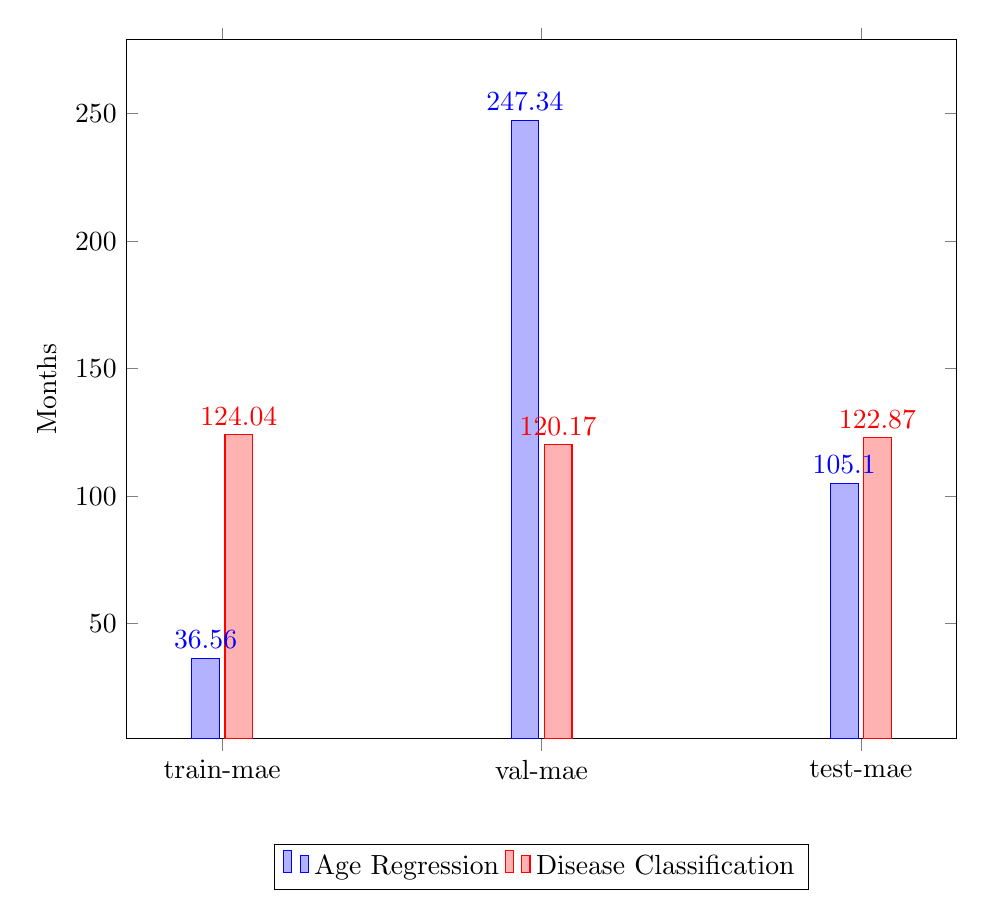
\begin{tikzpicture}
\begin{axis}[
    ybar,
    enlargelimits=0.15,
    legend style={at={(0.5,-0.15)},
    anchor=north,legend columns=-1},
    symbolic x coords={train-mae, val-mae, test-mae},
    ylabel=Months,
    xtick=data,
    nodes near coords,
    nodes near coords align={vertical}, 
    width=\linewidth
]
\addplot 
 coordinates {(train-mae, 36.5585) (val-mae, 247.3372) (test-mae, 105.0961)};
\addplot 
 coordinates {(train-mae, 124.0379) (val-mae, 120.1668) (test-mae, 122.8677)};
\legend{Age Regression, Disease Classification}
\end{axis}
\end{tikzpicture}
\caption{Impact of disease classification vs. age regression on chest dataset}
\label{fig:disease}
\end{figure}

For the training on the chest dataset, we noticed that within only 5 epochs the top-5 validation accuracy on the chest disease prediction rose to 73\%.


\subsubsection{Use chest samples within bone age range only}
The age range in the chest dataset varies across all ages. However the range in the bone age dataset is limited to 20 years. This test aimed at showing possible differences in performance when training the model with chest samples within age range of 0 to 20 only or with all samples.\\
The results are depicted in figure \ref{fig:maeagerange} showing the mean absolute error on the test set for either case.

\begin{figure}[H]
\centering
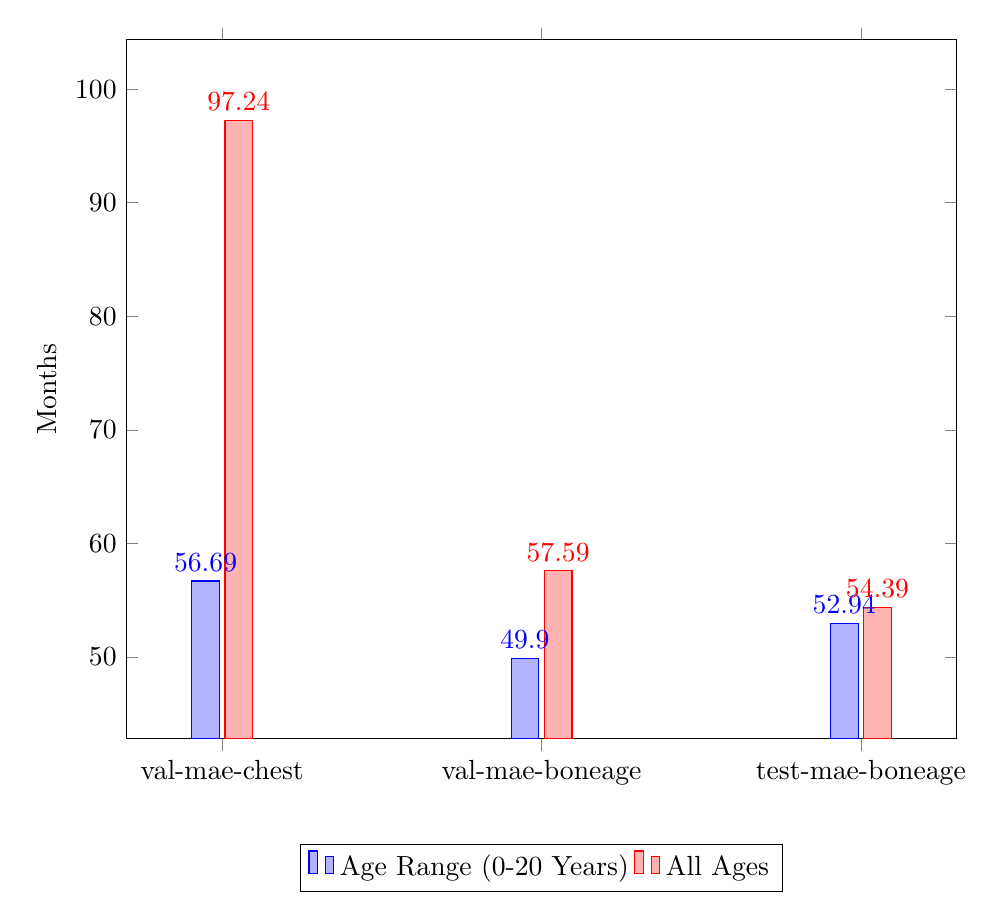
\begin{tikzpicture}
\begin{axis}[
    ybar,
    enlargelimits=0.15,
    legend style={at={(0.5,-0.15)},
    anchor=north,legend columns=-1},
    symbolic x coords={val-mae-chest, val-mae-boneage, test-mae-boneage},
    ylabel=Months,
    xtick=data,
    nodes near coords,
    nodes near coords align={vertical}, 
    width=\linewidth
]
\addplot 
 coordinates {(val-mae-chest, 56.6875) (val-mae-boneage, 49.9035) (test-mae-boneage, 52.9445)};
\addplot 
 coordinates {(val-mae-chest, 97.2429) (val-mae-boneage, 57.5860) (test-mae-boneage, 54.3883)};
\legend{Age Range (0-20 Years), All Ages}
\end{axis}
\end{tikzpicture}
\caption{Impact of reducing chest dataset to age range of bone age dataset}
\label{fig:maeagerange}
\end{figure}

The model trained on chest X-rays within the age range of 0 to 20 years only outperforms the other by 2.7\% and predicts the age with an 1.44 months better accuracy. This could be because the model gets more confused when it processes images from all ages rather than bone ages only. Also, perhaps the features of the chest change significantly as age increases. We also noticed that the size of the image set with the age range constraint was 15 times less than the size of the total set.

\subsubsection{Use different number of fixed layers in model}
In this experiment we used a fixed scenario except the number of trainable layers in the finetuning step increases with each test run by 10 from 10 to 90 layers. The architecture used was again \verb+InceptionV3+ as in the 'winner' model. The scenario included transfer learning on the chest dataset within the bone age range only and predicting patient age, and then finetuning of the model on the bone age dataset as in the previous experiment. Unfortunately we did not get the results in time as we repeatedly had difficulties with technical errors.

\subsubsection{Difference if model pretrained on ImageNet or not}
We wanted to know what quantitative difference it would make if the model used was not pretrained on ImageNet.  We used the 'winner' model and trained it on the bone age dataset. Two test runs, once the model is pretrained on ImageNet (i.e. with weights transferred) and once with random initialization only. The results are demonstrated in figure \ref{fig:pretrained}.

\begin{figure}[H]
    \centering
    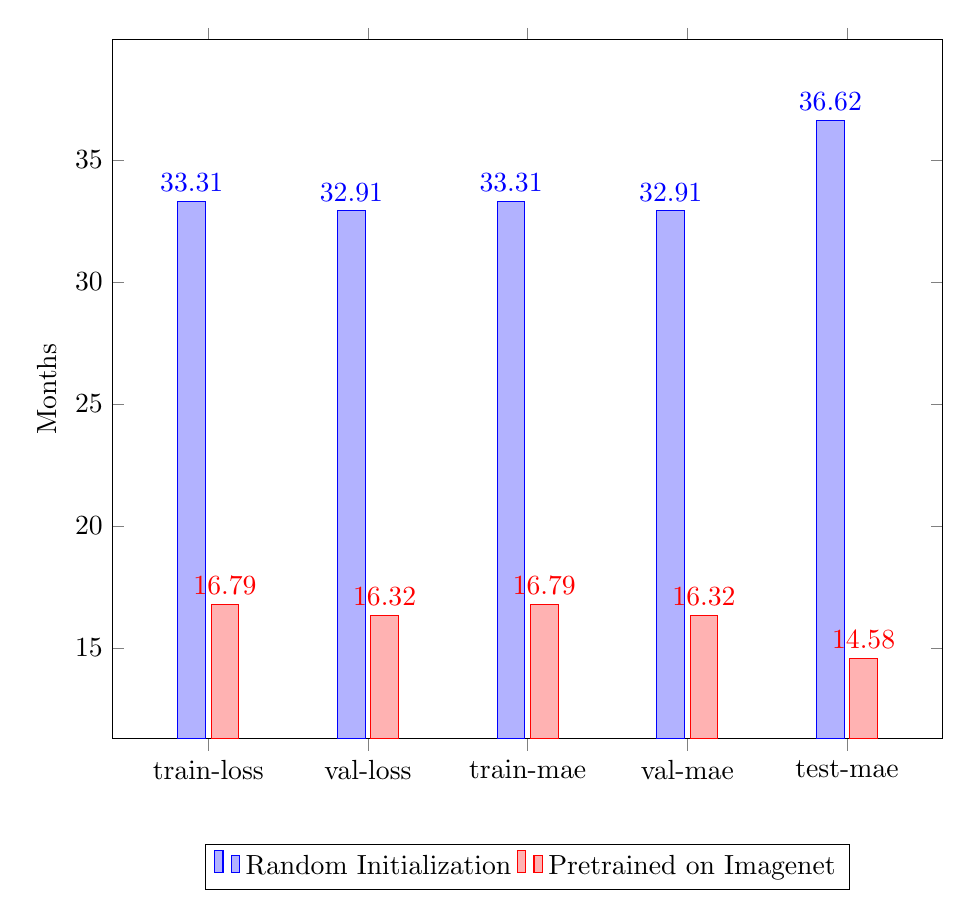
\begin{tikzpicture}
\begin{axis}[
    ybar,
    enlargelimits=0.15,
    legend style={at={(0.5,-0.15)},
    anchor=north,legend columns=-1},
    symbolic x coords={train-loss, val-loss, train-mae, val-mae, test-mae},
    ylabel=Months,
    xtick=data,
    nodes near coords,
    nodes near coords align={vertical}, 
    width=\linewidth
]
\addplot 
 coordinates {(train-loss,33.3080) (val-loss, 32.9127) (train-mae, 33.3080) (val-mae, 32.9127) (test-mae, 36.6205)};
\addplot 
 coordinates {(train-loss,16.7905) (val-loss, 16.3172) (train-mae, 16.7905) (val-mae, 16.3172) (test-mae, 14.5822)};
\legend{Random Initialization, Pretrained on Imagenet}
\end{axis}
\end{tikzpicture}
\caption{Impact of pretrained model versus random initialization}
\label{fig:pretrained}
\end{figure}

It is plain to see that the model performs much better when it is pretrained with ImageNet instead of random initialization. We think that to some extent the low level features from the ImageNet dataset are similar to those in the X-rays images and therefore the pretrained model performs much better as it already nows the low level features of the images.

\subsubsection{Does including gender as input improve the result?}
While the 'winner' model incorporated the patient gender into their model, we wanted to demonstrate experimentally if the difference in performance was observable and significant. For that we used the 'winner' model and trained it on the bone age dataset once with the gender as input and once without (i.e. only the image) and compared the performances. Figure \ref{fig:gender} shows the results.

\begin{figure}[H]
    \centering
    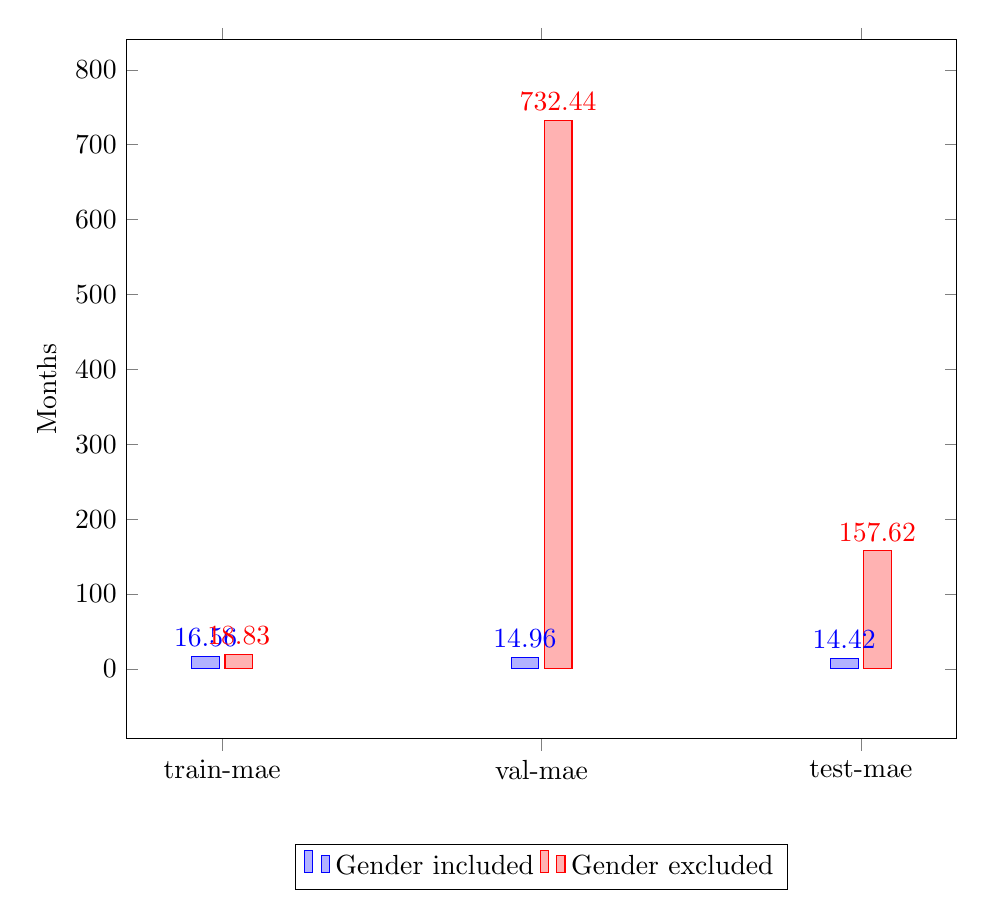
\begin{tikzpicture}
\begin{axis}[
    ybar,
    enlargelimits=0.15,
    legend style={at={(0.5,-0.15)},
    anchor=north,legend columns=-1},
    symbolic x coords={train-mae, val-mae, test-mae},
    ylabel=Months,
    xtick=data,
    nodes near coords,
    nodes near coords align={vertical}, 
    width=\linewidth
]
\addplot 
 coordinates {(train-mae, 16.5583) (val-mae, 14.9614) (test-mae, 14.4218)};
\addplot 
 coordinates {(train-mae, 18.8303) (val-mae, 732.4419) (test-mae, 157.6202)};
\legend{Gender included, Gender excluded}
\end{axis}
\end{tikzpicture}
\caption{Impact of adding gender as input on the prediction performance}
\label{fig:gender}
\end{figure}

While some numbers appear somewhat confusing, in each case the gender adds a distinct advantage to the performance. The high values might be due to the low number of epochs used. Confer the validation loss spikes in figure \ref{fig:lossSeResNet50}.

\subsubsection{Regression vs. classification on age}
In this experiment the aim was to analyze the effect of the architecture of the last layer on the performance. We ran two tests with the 'winner' model on the bone age dataset. In the first test the last layer of the model was a dense layer with one output to predict the age as a regression problem. In the second test the last layer consisted of a 240 neuron dense layer representing a classification problem to predict the age between 0 and 240 months. Results are shown in table \ref{table:classvsreg}. For classification we used top-1 and top-5 accuracy. Given our normal regression performance of 10 to 20 months we could have experimented with \eg top-10 or top-20 accuracy as well. As there is an almost 5 fold increase in accuracy from top-1 (8\%) to top-5 (35\%) it could well be that top-10 accuracy is around 65\%. Continuing this, top-20 accuracy would be around 100\%. But this is pretty plausible: Given the regression performance of around 10 months on average (table \ref{table:archcomp}) top-20 accuracy could cover 10 months in either direction.

\begin{table}[H]
\centering
\caption{Classification versus Regression}
\label{tab:classificationRegression}
\scalebox{0.85}{
\begin{tabular}{l|rrrr}
               & val-loss & val-top-1-acc & val-top-5-acc & val-mae \\ \hline
class. top-1   & 5.5084   & 0.0821        &               &         \\
class. top-5   & 9.4924   &               & 0.3502        &         \\
regression     & 18.1380  &               &               & 18.1380
\end{tabular}
}
\label{table:classvsreg}
\end{table}


\subsection{Comparison to baseline}
The 'baseline' model has a validation MAE of 13.91 months according to \cite{kaggleboneage}.

\subsubsection{Pretrain baseline \cite{kaggleboneage} with NIH chest dataset}
We took the 'baseline' model and first trained it on the large NIH chest dataset (predicting patient age) to see if it would perform better in the bone age prediction task. Finetuning was used on the bone age dataset with no additional layers freezed. \\
Our test run achieved a MAE of 17.27 which fell a bit short of our expectation. However we trained it for only 5 epochs, the result could likely change if trained much longer.

%------------------------------------------------------------------------
\section{Conclusions}
None of our image preprocessing attempts caused notable improvement. The use of different architectures demonstrated that performance gains are possible but it requires further investigation to draw conclusions. Likewise, we experimented with transfer learning on the chest dataset and reused the weights for age prediction on the pediatric X-rays. While we were able to show significant improvements between some sets of hyperparameters, at this point we cannot conclude whether the use of the large chest dataset towards transferring knowledge to the bone age prediction task actually does bring a distinct advantage or not. This question should be investigated further as part of future work.

\subsection{Future work}
\subsubsection{Experiment with combination of best results}
Combine all the best results into one architecture and model, respectively, and train it for 500 epochs just like they did for the winners model. This would include 
\begin{itemize}
\item use SeResNet50 or InceptionV3 model
\item use gender as additional input to image
\item use age regression on chest dataset for TL
\item use NIH chest samples only within bone age range
\item use model pretrained on ImageNet
\end{itemize}

In general, run the experiments with much more epochs as we used only a very small number.

\subsubsection{Ensemble learning}
Experiments using ensemble learning could lead to better prediction performance.

\subsubsection{Hyperparameter tuning}
We did not systematically try to find a set of optimal hyperparameters for the models. For instance, one could invest in that direction with a grid search.

\printbibliography

\end{document}
